\documentclass[12pt]{article}
%\usepackage{graphicx}
\usepackage{indentfirst}
\usepackage[export]{adjustbox}
\usepackage{graphicx}
\usepackage{float}
\usepackage{hyperref}
\usepackage{makecell}

%opening
\title{Audio effects library\\Project schedule and communication plan}
\author{Kacper Harezga, Ewa Kobiela, Jan Laskowski\\Krzysztof Sobczyk, Grzegorz Machura}
\date{24.04.2021}
\begin{document}
	
	\maketitle
	\tableofcontents
	\newpage
	
\section{Plan schedule management}

	The process of developing the project schedule consists of defining the activities that will be needed to fulfill the project scope, estimate duration of specific tasks and prepare a schedule based on these information.
	
	The rocess of schedule creation and management is presented in this document. All files and work used in the process is mentioned in the document or attatched as attatchement.

\section{Define activities}

	In order to produce project deliverables, specific work packets needs to be defined. Below we will recall work breakdown structure document followed by the dictionaty which explains the scope of each work package. Using the WBS document we define activities that will be performed during the process of project creation.
	
	The five main segments that needs to be fulfilled include:
	\begin{itemize}
	\item research - collecting information and learning about digital signal processing in Python. At this stage we prepare for implementing the effects
	\item time-domain effects and frequency domain effects - this is the main stage of the project. During this part we implement various types of filters and create the library of audio effects
	\item creating signal path - in order to present the usage of the library, we create a full signal path, which allows user to add chosen effect to input audio signal
	\item testing - finally, the library and signal path application will be tested to prove it can be used by the user
	\end{itemize}
	
	\begin{figure}[H]
		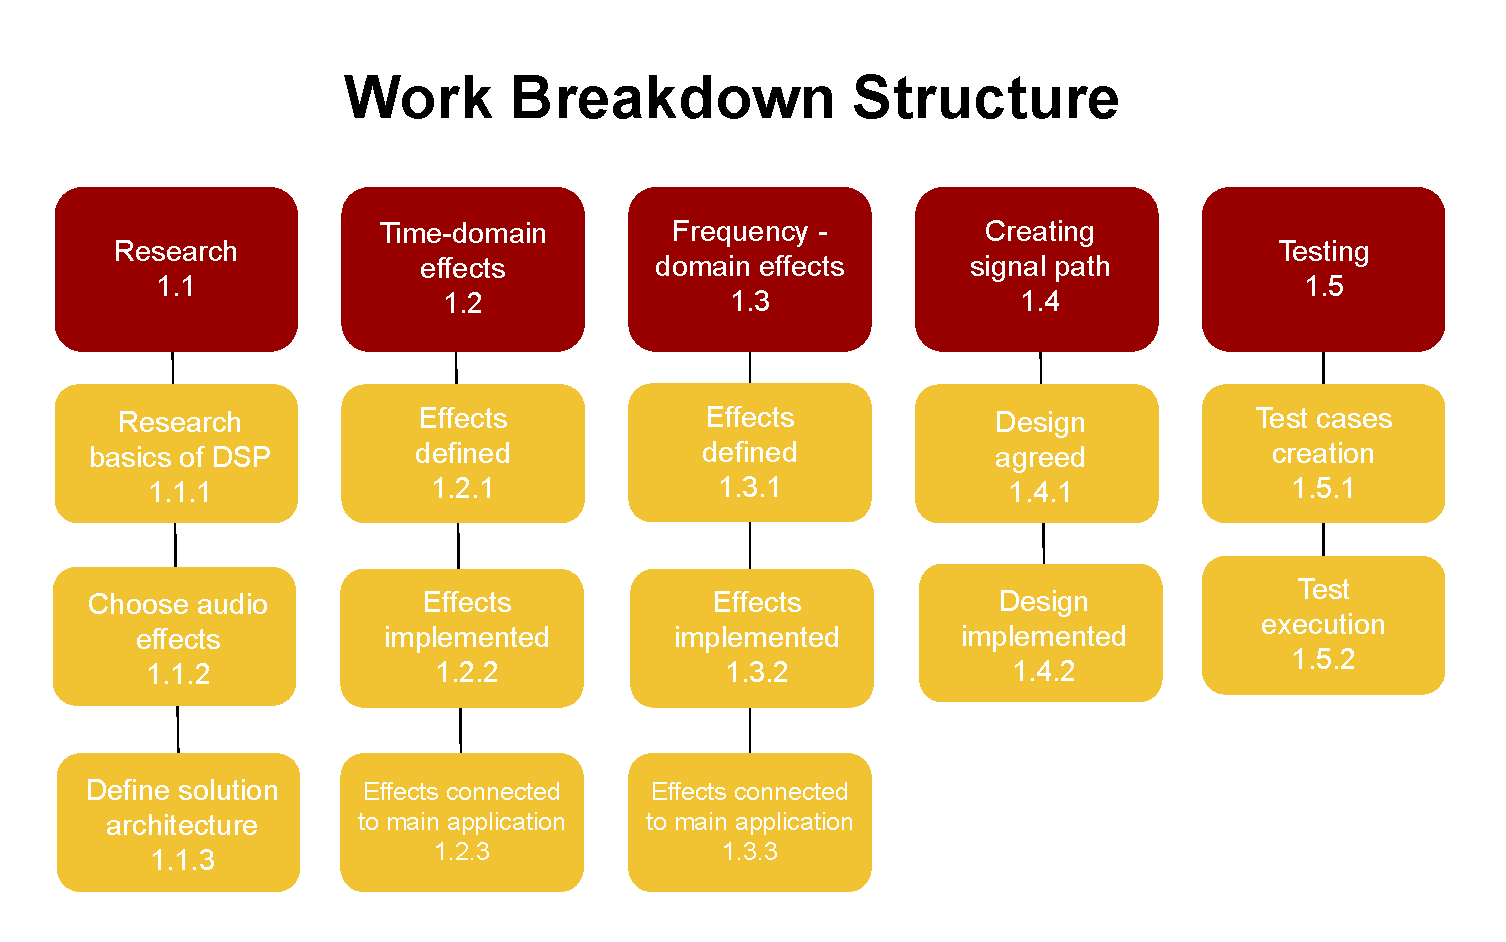
\includegraphics[width=1.2\textwidth, center]{WBS}
		\caption{Work breakdown structure}
	\end{figure}
	\begin{figure}[H]
		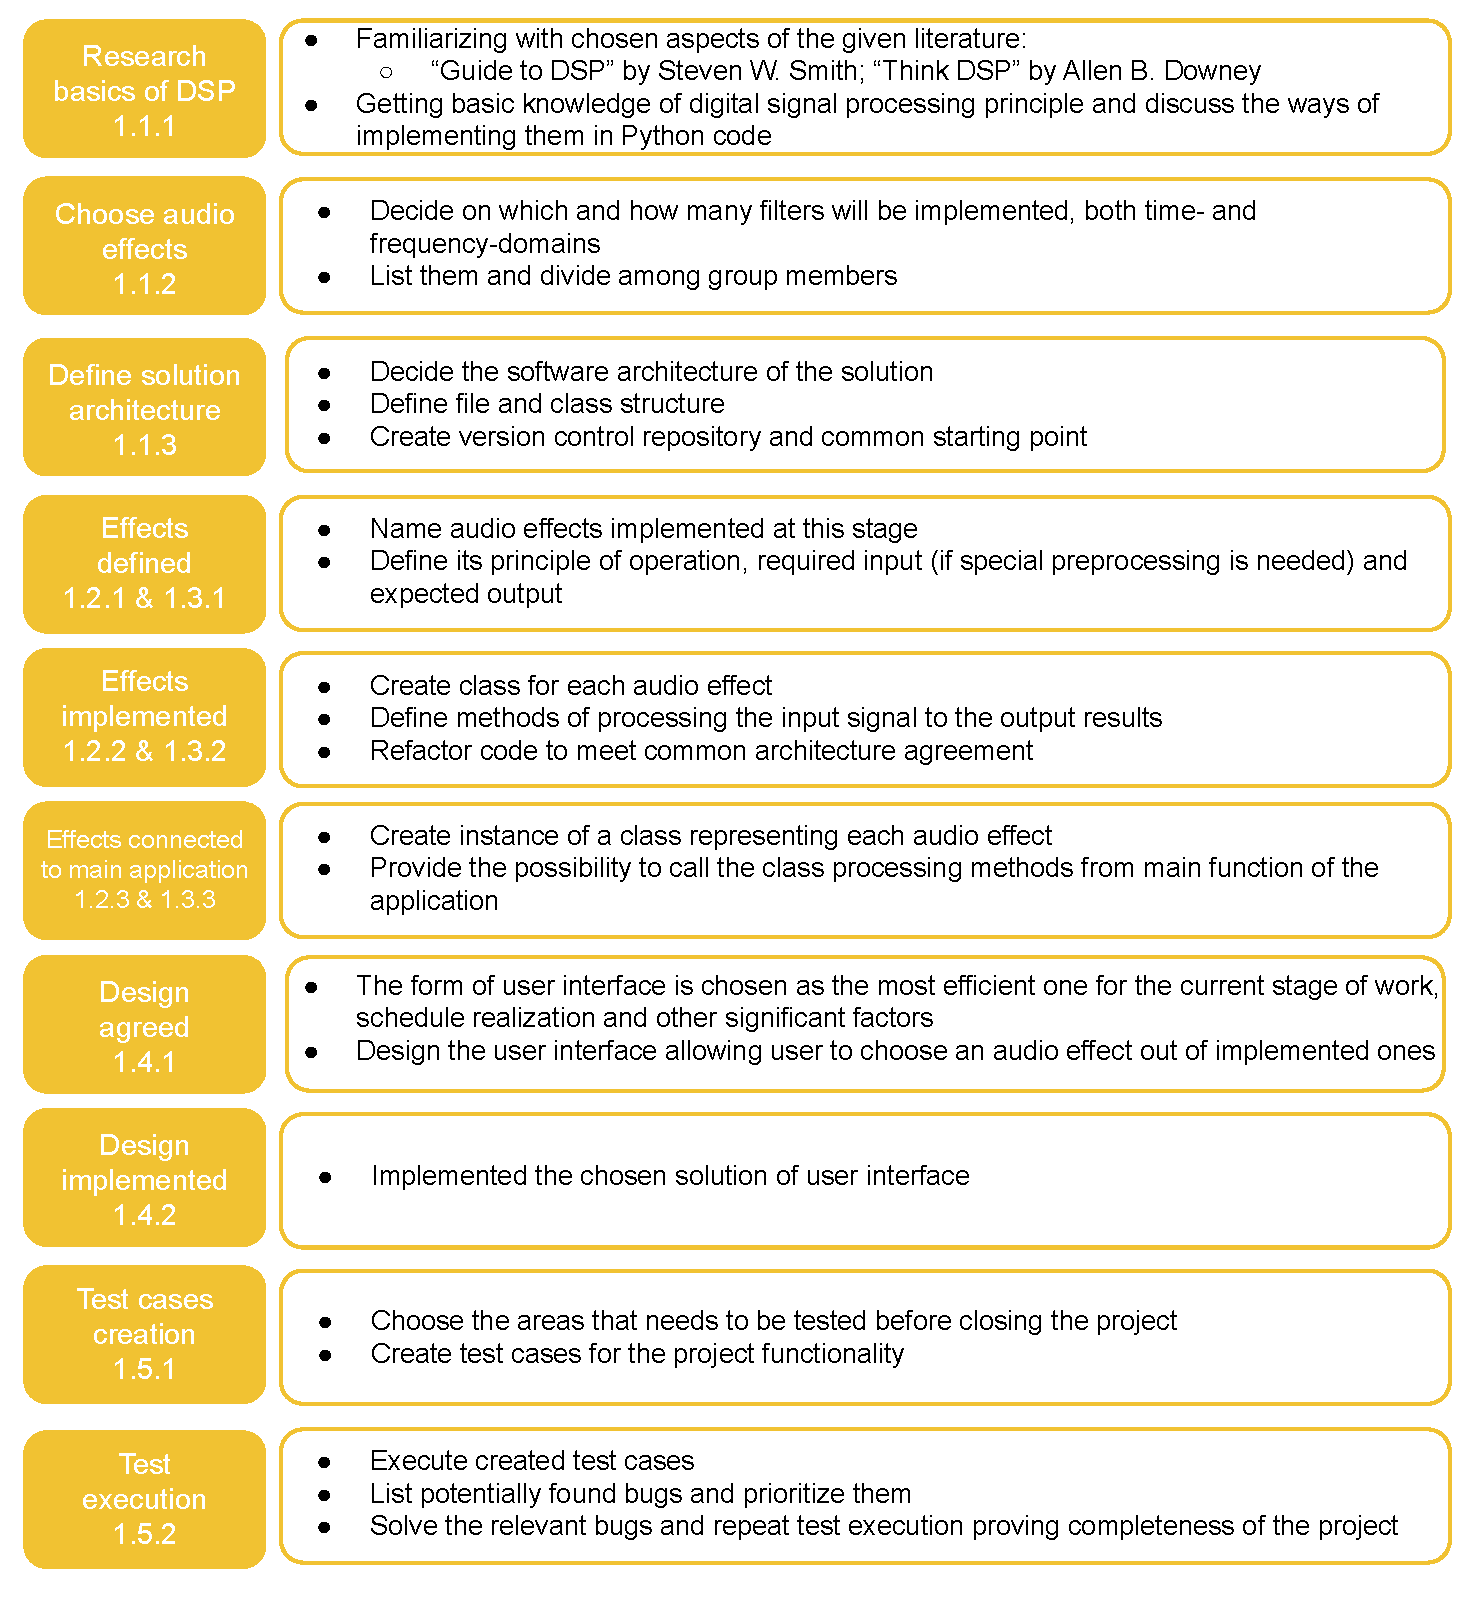
\includegraphics[width=1.2\textwidth, center]{WBS dictionary}
		\caption{Work breakdown structure dictionary}
	\end{figure}

\section{Sequence activities}

	The sequence activities diagram below represents relations and interaction between project objects in sequential order. This diagram consists of four objects: the user, directory, libraty and methods of the filter class.
	
	Firstly, the user needs to save the input file into predefined directory. Then they will choose in library an audio effect to be applied. Having these presonditions, the library reads input file from the directory and calls processing node function frm choosen audio effect class. In the class file the effect is added to the base signal and the class returns .wav file. The file is written into the directory by the library. Finally, user can collect the processed file.
	
	\begin{figure}[H]
		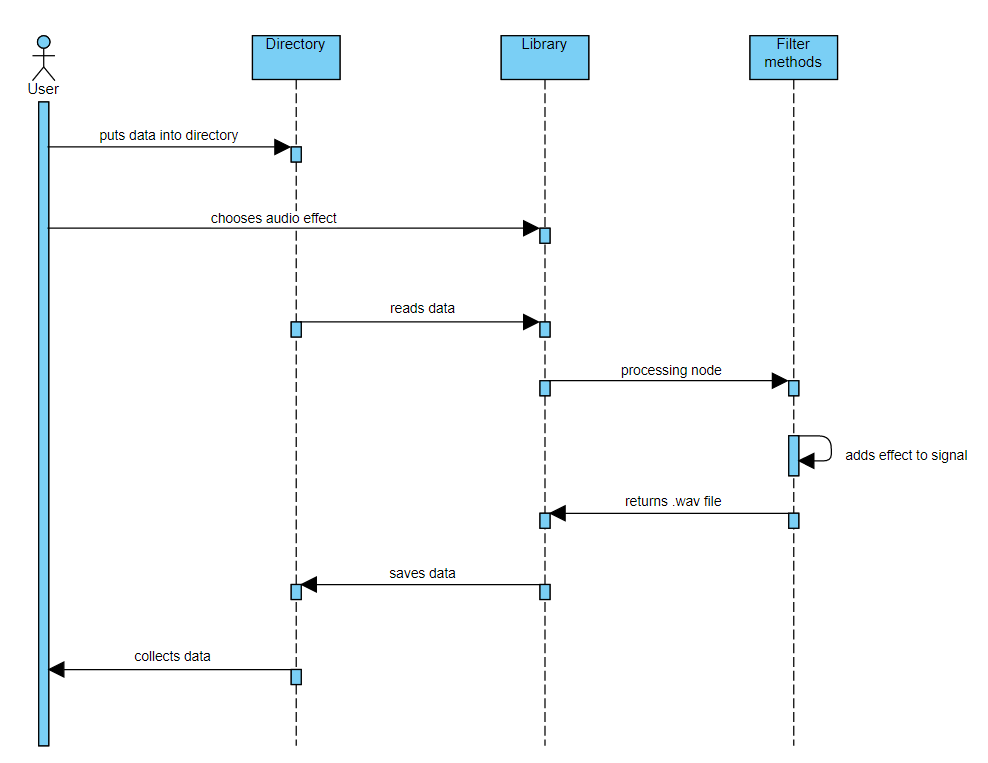
\includegraphics[width=1\textwidth, center]{Sequence activities diagram}
		\caption{Sequence activities diagram}
	\end{figure}

\section{Estimate activity durations}

	The process of estimating schedule of the project is based on work patkets defined in work breakdown structure documment, which we also call tasks or activities. Using defined activities we predict how much time will they consume:
	
	\begin{itemize}
	\item Research basics of DSP - 2 weeks
	\item Choose audio effects - 1 week
	\item Define solution architecture - 2 weeks
	\item Define effects (both time- and frequency-domain) - 1 week per each
	\item Implement effects (both time- and frequency-domain) - 2 weeks per each
	\item Connect effects classes to common signal path (both time- and frequency-domain) - 1 week per each
	\item Agree on design of user interface - 2 weeks
	\item Implement user interface - 2 weeks
	\item Create test cases - 3 days
	\item Execute test cases - 3 days
	\end{itemize}

\section{Develop schedule}

	According the the estimated duration of activities the schedule was developed. We tried to execute tasks one by one, however due to the fact that the project should be finished in 14 weeks and total estimated time for all tasks is equal 18 weeks, we allowed some overlapping. Thus we decided that time and frequency-domain filters will be implemented in parallel by different members and stakeholders will be notified when approximately half of them are ready. We will also inform Dolby company after finishing each of five segments.
	
	The Gant chart with activities scheduled in weekly intervals is presented below. Applying the weekly approach also allows us to plan weekly meetings in which we can discuss progress from previous week - as each week either one work package will be finished or halfway done.

\begin{figure}[H]
		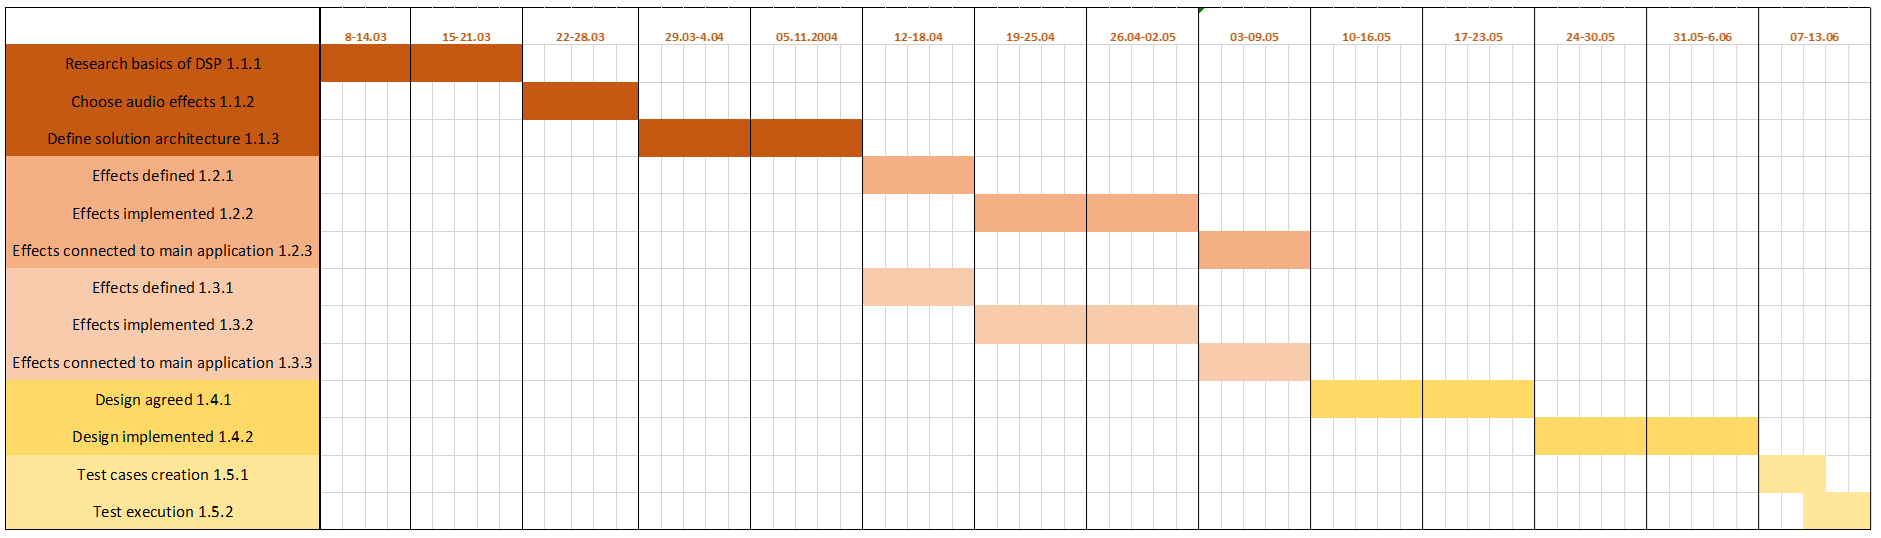
\includegraphics[width=1.1\textwidth, center]{Gant chart}
		\caption{Gant chart}
	\end{figure}

\section{Communication plan}
	
	The communication between the project team and stakeholders will be conducted via e-meetings. The Dolby company proposed their own BlueJeans communication tool which we will use to present progress of the project and receive feedback. In the communication with the university party we will be using Microsoft Teams. For internal communication we will be using instant messaging in Facebook Messenger and the meetings will be conducted in Discord application.
	
	Language using in internal communication and communication with Dolby is Polish, for both official and unofficial docummentation. However, the project docummentation must be written in English due to the language in which the university course is conducted. However the informal communication may be handled in Polish.
	
	We do not specify any dates or frequency of meetings with both primary stakeholders. The plan assumes that the project members will reach a meeting request and the project manager will contact the stakeholder via email message and establish the meeting time. During the meeting we will discuss improvements or progress, ask for further information or explaining of technical matters or rise questions.
	
	The plan also assumes frequent team meetings, occuring each weekend in the form of catch-up on individual progresses and report any problems or blockers occuring up to date.
	
\end{document}